\chapter{Introduction}
The \emph{min--max principle} is a unifying theme across analysis, geometry, and topology. At its core, it provides a strategy for identifying critical values of a functional by working not with single points, but with continuous families of points. One begins with a \textbf{space of objects} (often a function space), chooses a $p$-parameter \textbf{admissible family} of objects (typically forming a continuous submanifold of the space), evaluates a \textbf{functional} along this family, and records the unavoidable peak value - the \textbf{mountain to be crossed}. This is the essence of the \emph{mountain--pass algorithm}.  

The simplest case is $p=1$: a single path through the space. One can imagine the path as a string of balls connected by a thread, draped across a valley. Under gradient descent, each ball rolls downhill, but because they are tied together, some fall to one side, some to the other and at least one remains suspended at the saddle point across the valley floor. That ball marks a critical point of the functional. In higher dimensions, the same idea applies with $p$-parameter families: the greater the dimensionality of the family, the higher the ``mountain'' it is forced to cross. 

This perspective appears in many guises. In linear algebra, it underlies the variational characterisation of the eigenvalues of real symmetric matrices. In geometry, min--max methods are central to the construction of closed geodesics (Birkhoff \cite{Birkhoff27}) and minimal hypersurfaces (Almgren \cite{Almgren62}, Pitts \cite{Pitts81}, Marques--Neves \cite{MarquesNeves14}, \cite{MarquesNeves17}). In the study of nonlinear PDEs, mountain--pass arguments provide existence results for critical points of variational functionals (Guaraco \cite{Guaraco18}), such as the Allen--Cahn energy (Gaspar--Guaraco \cite{Guaraco16}).  

Although these applications are often studied in isolation, they share a unifying intuition: any continuous deformation within a constrained space must inevitably pass through certain “bottlenecks,” and these bottlenecks encode fundamental invariants of the system. This dissertation develops this theme in three domains of decreasing familiarity in the literature: first, the classical setting of linear spectral theory; second, the more recent framework of planar widths (Guth \cite{Guth07}); and third, the variational study of PDEs such as the Allen--Cahn equation.

 
\section{Overview and Key Results}
In Chapter \ref{ch:2}, we reinterpret the spectral theorem for real symmetric matrices through the min--max lens. In this case, the elements of the mountain--pass algorithm are the following: the \textbf{points in the space} are vectors in $\mathbb{R}^n$; the \textbf{admissible families} are $p$-dimensional linear subspaces intersected with the unit sphere; the \textbf{functional} is the \emph{Rayleigh quotient}, defined on $S^{n-1}\subset\mathbb{R}^n$; and the \textbf{mountains to be crossed} are the successive eigenvalues. The first eigenvalue arises simply by minimising the Rayleigh quotient over $S^{n-1}$. The second eigenvalue, however, cannot be obtained by direct minimisation; instead, it is characterised by taking all two-dimensional linear subspaces (whose intersections with $S^{n-1}$ are great circles), computing the maximum Rayleigh quotient along each, and then minimising over all such families. Higher eigenvalues are obtained analogously by considering $p$-dimensional subspaces, taking the maximum of the Rayleigh quotient over their intersections with $S^{n-1}$, and minimising over all such choices. This is summarised by the following theorem:
\begin{quote}
\textbf{Theorem \ref{CourantFischer} (Courant--Fischer Min--Max - linear setting).}  For a real symmetric matrix $A \in \mathbb{R}^{n \times n}$ with ordered eigenvalues $\lambda_1 \leq \cdots \leq \lambda_n$, the $k^{\text{th}}$ eigenvalue admits the min--max characterisation: $$\lambda_k=\min_{\substack{L\subset \mathbb{R}^n\\ \dim L = k}} \max_{\substack{\vec{v}\in L\\ \vec{v}\neq 0}} R(\vec{v}),$$
where $R:\mathbb{R}^n\setminus\{0\}\to \mathbb{R}$ is the Rayleigh quotient, $R(\vec v)=\dfrac{\langle \vec {v}, A\vec{v}\rangle}{\langle\vec v,\vec v\rangle}$.
\end{quote}
This is the linear prototype of the mountain--pass principle: eigenvalues arise as a progression of successive “mountain--passes,”  each forced by the dimensionality of the admissible families.\\
Building on this, we turn to \emph{homology} as a more flexible framework for organising admissible families in nonlinear settings. Linear subspaces tell directions apart using orthogonality, homology tells loops apart by how they \emph{wind}. Two closed curves are the same in homology if one can be slid into the other without cutting. On a torus there are two basic ways to go around (meridian and longitude), so any closed curve is determined, up to such sliding, by two integers \((m,n)\) counting how many times it winds in each direction. More compactly, \(H_1(T^2)\cong \mathbb{Z}\oplus\mathbb{Z}\). Replacing the linear subspaces in Courant--Fischer by homological cycles, we index admissible families by nontrivial classes in $H_p$. We now obtain min--max values because a nonzero class cannot be contracted to the trivial one within the admissible category.

\noindent \emph{Morse theory} refines this picture, relating the topology of the underlying space (say, the sphere carrying the Rayleigh quotient) to the number and indices of critical points: 
\begin{quote}
\textbf{Theorem \ref{MorseIneq} (Weak Morse Inequality).}
Let $M$ be a compact manifold and let $f:M\rightarrow R$ be a Morse function. Denote by $c_k \in \mathbb{N}$ the number of critical points of $f$ with index $k$, on $M$. Then
$$\beta_k(M) \leq c_k,$$
where $\beta_k(M) := \dim H_p(M;\mathbb{Z}_2)$ is the $k^{\text{th}}$ \emph{Betti} number of $M$. These inequalities show that nontrivial homology classes force the existence of critical points at the corresponding indices.
\end{quote}
In this sense, homological cycles replace linear subspaces, giving independent “directions of deformation” that produce robust mountain--pass levels. This perspective suggests running min--max over homology classes, giving a broad nonlinear analogue of the spectral framework.

\noindent Chapter \ref{ch:3} develops the geometric analogue via the notion of $p$-\emph{widths}, a nonlinear spectrum built using the min--max algorithm over families called sweep--outs. We focus on the \emph{first width} $(p=1)$ for planar domains. Informally, the simplest $1$-parameter sweep--out on the disc is given by a family of parallel chords. We use the horizontal chords out of convenience. 
\begin{figure}[ht]
  \centering
  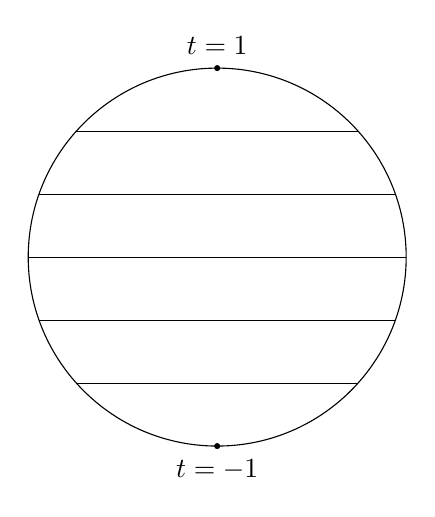
\begin{tikzpicture}[line cap=round]
    \tikzset{pole/.style={circle, fill=black, inner sep=0pt, minimum size=2.2pt}}
  % parameters
  \def\R{2.4}      % radius (cm)
  \def\N{5}        % number of chords

  % compute spacing so chords don't sit on the boundary
  \pgfmathsetmacro{\step}{2*\R/(\N+1)}

  % draw chords inside the circle
  \begin{scope}
    \clip (0,0) circle (\R);
    \foreach \i in {1,...,\N} {
      \draw (-\R-0.3, -\R + \i*\step) -- (\R+0.3, -\R + \i*\step);
    }
  \end{scope}

  % circle outline last so it sits on top
  \draw (0,0) circle (\R);

  \node[pole, label={above:$t=1$}]   at (0,\R)   {};
  \node[pole, label={below:$t=-1$}]  at (0,-\R)  {};
\end{tikzpicture}

  \caption{Reference sweep--out by horizontal chords $\{\gamma_t^*\}_{t\in[-1,1]}$.}
\end{figure}
\FloatBarrier

\noindent For general disc--like domains, such as convex polygons, we understand a sweep--out as a continuous deformation of such a family. To make sweep-outs topologically nontrivial, we impose the condition that the map at the boundary has winding number 1. 
\begin{figure}[ht]
  \centering
  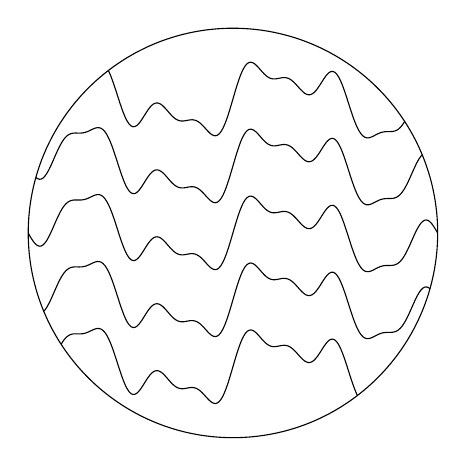
\begin{tikzpicture}[line cap=round]
  % parameters
  \def\R{2.6}   % disk radius
  \def\N{7}     % number of chords
  \def\t{1.0}   % 0 = straight chords, 1 = fully deformed
  \def\A{0.38}  % deformation amplitude (relative to R)

  % spacing of the reference chords
  \pgfmathsetmacro{\step}{2*\R/(\N+1)}

  % a smooth x-only warp (so ordering in y is preserved => no crossings)
  \pgfmathdeclarefunction{warp}{1}{%
    % argument is x/R (dimensionless). trig in radians -> add 'r'
    \pgfmathparse{0.35*sin(2*pi*#1 r) + 0.22*sin(5*pi*#1 r + 0.7) + 0.12*sin(9*pi*#1 r - 0.4)}%
  }

  \begin{scope}
    \clip (0,0) circle (\R);
    \foreach \i in {2,3,4,5,6} {
      \pgfmathsetmacro{\c}{-\R + \i*\step} % reference y-level
      \draw plot [smooth, samples=220, domain=-\R:\R]
        (\x, { \c + \t * \A * \R * warp(\x/\R) + 0.2*(\i-4)});
    }
  \end{scope}

  % boundary last
  \draw (0,0) circle (\R);
\end{tikzpicture}

  \caption{General sweep--out $\{\gamma_t\}_{t\in[-1,1]}$ on the disc .}
\end{figure}
\FloatBarrier

\noindent With this picture in mind, the first width is
\begin{equation}
    \omega_1(\Omega)=\inf_{(\{\gamma_t\})}\ \sup_{t\in[-1,1]}\mathrm{Length}(\gamma_t),   
\end{equation}

the least possible largest length among such sweep--outs. In this case, the elements of the mountain--pass framework are the following: the \textbf{points in the space} are submanifolds of a fixed domain; the \textbf{admissible families} are $1$-parameter \emph{sweep--outs} whose union covers the domain; the \textbf{functional} is the length of curves in the sweep--out; and the \textbf{mountain to be crossed} is the first width. Courant--Fischer characterises the second eigenvalue as follows: for each $2$-dimensional linear subspace $L\subset\mathbb{R}^n$ (so $L\cap S^{n-1}$ is a great circle), take the maximum of the Rayleigh quotient on $L\cap S^{n-1}$; then minimise this maximum over all such $L$. The first width is the analogous nonlinear construction: for each $1$-parameter family of curves (a sweep–out), take the maximum length occurring in the family; then minimise this maximum over all sweep–outs. In this sense $\{\omega_p\}$ acts as a nonlinear spectrum with $\omega_1$ playing the role of a “second eigenvalue” for the length functional. In this section we present a \textbf{novel proof}, based on a topological argument, of the first width of convex polygons: 
\begin{quote}
\textbf{Theorem \ref{thm:first-width-convex-polygon} (First width of convex polygons).}
Let $P\subset\mathbb{R}^2$ be a compact convex $n$-gon with edges $E_1,\dots,E_n$ and vertices $V_1,\dots,V_n$ labelled clockwise, cyclically. The first width equals the minimal distance between two parallel supporting lines of $P$:
\[
\omega_1(P)
= \min_{\|\vec{u}\|=1} \big( \max_{\vec{x}\in P} \vec{x}\!\cdot \vec{u} - \min_{\vec{x}\in P} \vec{x}\!\cdot \vec{u} \big)
= \begin{cases}
        \displaystyle \min_{1\le i\le n}\ \operatorname{dist}\!\big(V_i,E_{V_i}^{\mathrm{opp}}\big), & \text{if $n$ is odd},\\
        \displaystyle \min_{1\le i\le n}\ \operatorname{dist}\!\big(E_i,E_{E_i}^{\mathrm{opp}}\big), & \text{if $n$ is even}.
    \end{cases}
\]
Here $E_{V_i}^{\mathrm{opp}}$ denotes the unique edge opposite the vertex $V_i$ when $n$ is odd, and $E_{E_i}^{\mathrm{opp}}$ denotes the unique 
edge opposite $E_i$ when $n$ is even. For a triangle this reduces to “$\omega_1 =$ smallest altitude.”
\end{quote}
While the equality itself is known in the literature (see \cite{Chodosh25}), our contribution is providing a \emph{new proof} that the minimal distance between opposite supports is a lower bound for the first width. The main idea in our method, which can be found in Lemma (\ref{lem:polygon-width-ub}), is to track endpoints of the curves throughout the sweep--out, view their evolution as a loop on the torus, and designate a target set on the torus (another loop) that realises the claimed width. By known results on the intersection number of loops on $T^2$, the endpoint loop meets this target set, forcing a curve of length at least the claimed value (lower bound). A matching upper bound comes from a parallel--line sweep--out that attains this distance. This viewpoint is flexible and suggests extensions to other sweep--out and width problems, which we discuss in the Further Directions, Chapter \ref{ch:5}.

\noindent Finally in Chapter~\ref{ch:4}, we consider a third problem in the mountain--pass setting. In this case, the elements of the mountain--pass algorithm are as follows. The \textbf{points} are functions in an appropriate Hilbert space. The \textbf{admissible families} are smooth $p$-parameter families in that space. The \textbf{functional} is the \emph{Allen--Cahn energy}
\[
E_\varepsilon(u)=\int_{\Omega} \frac{\varepsilon}{2}\,|\nabla u|^2+\frac{1}{\varepsilon}W(u),
\]
whose Euler--Lagrange equation is the Allen--Cahn PDE
\[
-\varepsilon\,\Delta u+\frac{1}{\varepsilon}\,W'(u)=0 \quad \text{in } \Omega.
\]
The \textbf{mountains} are the nontrivial critical values of this energy obtained via such families.Concretely, fix a smooth double--well potential $W$ and let $c_\varepsilon$ denote the associated min--max critical level. Guaraco showed that, after the natural Modica--Mortola rescaling,
\[
\frac{1}{2\sigma}\,c_\varepsilon\ \longrightarrow\ \omega_1(\Omega)\qquad(\varepsilon\to 0),
\qquad
\sigma=\int_{-1}^{1}\sqrt{2W(s)}\,ds,
\]
thereby providing a PDE realisation of geometric widths and a route to minimal hypersurfaces via Allen--Cahn. Geometrically, the min--max solution $u_\varepsilon$ develops a thin transition layer where $u_\varepsilon$ crosses between the wells; as $\varepsilon\to 0$ the level sets (e.g. $\{u_\varepsilon=0\}$) concentrate on a rectifiable curve $\Gamma\subset\Omega$ that is stationary for length and satisfies $\mathrm{Length}(\Gamma)=\omega_1(\Omega)$. In other words, the Allen--Cahn interfaces ‘draw’ the width–realising curve in the small–$\varepsilon$ limit, with $E_\varepsilon(u_\varepsilon)/(2\sigma)\to \mathrm{Length}(\Gamma)=\omega_1(\Omega)$.

Our focus here is twofold: \emph{theoretically}, we make this correspondence precise by discussing that transition layers of min--max Allen--Cahn solutions converge, as $\varepsilon\to 0$, to curves realising the widths of $\Omega$; and \emph{computationally}, we complement this with two numerical implementations of the mountain--pass principle—(i) for the area functional, discretising a cylindrical domain by a triangular mesh and running a mountain--pass algorithm on the area viewed as a function of vertex positions, thereby obtaining discrete saddle--type critical points such as the catenoid; and (ii) for the Allen--Cahn energy, approximating the infinite--dimensional function space by a finite--element discretisation and computing nontrivial critical points via an analogous mountain--pass search. In parallel with Guaraco’s theorem—showing that Allen--Cahn min--max energies converge (after rescaling) to geometric widths—our computed min--max energies reflect these underlying geometric invariants. Taken together, these experiments demonstrate how the min--max framework can be made computational, linking discrete algorithms with the analytic and geometric theory.
